% !TeX spellcheck = en_GB
% ***************************************************** %
\section{Results}\label{subsc:res}
% ***************************************************** %

Firstly we explore the \emph{solution space} using the \texttt{multi-start} meta-heuristics on different TSP instances, the we solve another instance of the problem and we show the results in figures~\ref{fig:res-local-search} and~\vref{fig:res-sim-annealing}.


% ***************************************************** %
\subsection{Energy landscape}\label{subsc:energy-land}
% ***************************************************** %





%\begin{figure}
%\centering
%\subfloat[]%
%	{} \,
%\subfloat[]%
%	{}
%\caption{Local search and SA energy view}
%\label{fig:res-energy}
%\end{figure}



\begin{figure}
\centering
\subfloat[\emph{\texttt{swap} method on circular layout}]%
	{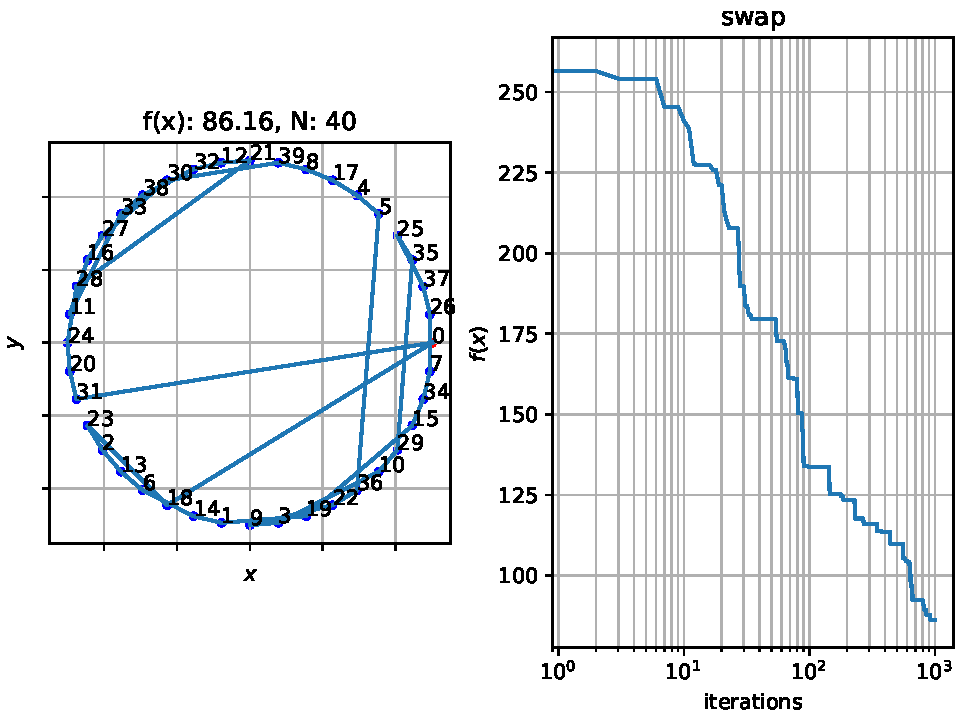
\includegraphics[width=0.49\textwidth]{circle-swap}} \,
\subfloat[\emph{\texttt{reverse} method on circular layout}]%
	{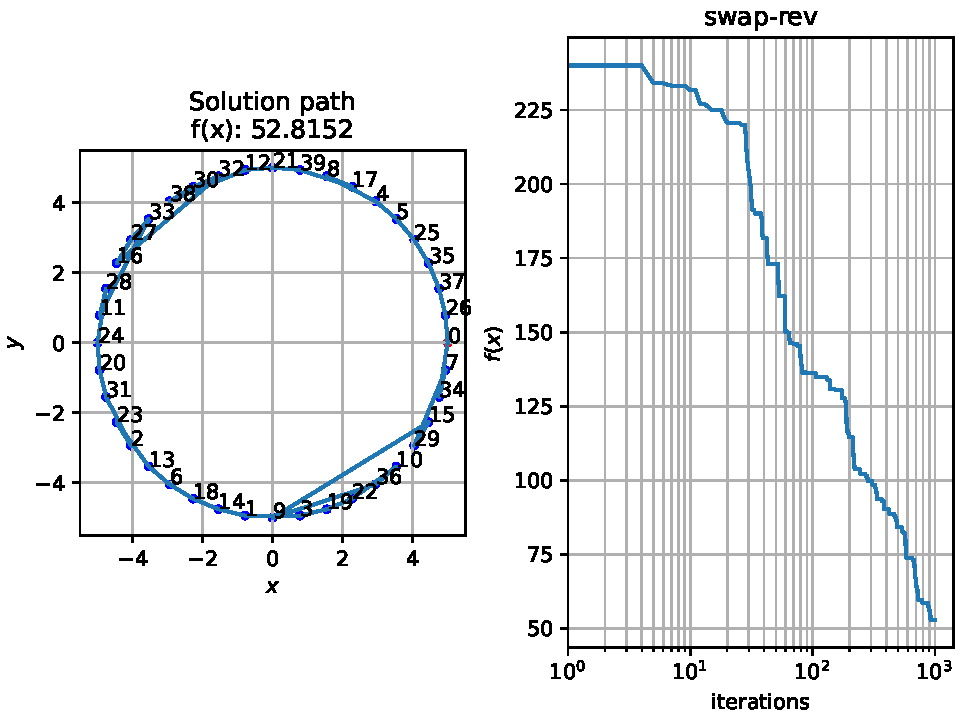
\includegraphics[width=0.49\textwidth]{circle-swaprev}} \\
\subfloat[\emph{\texttt{swap} method on random layout}]%
	{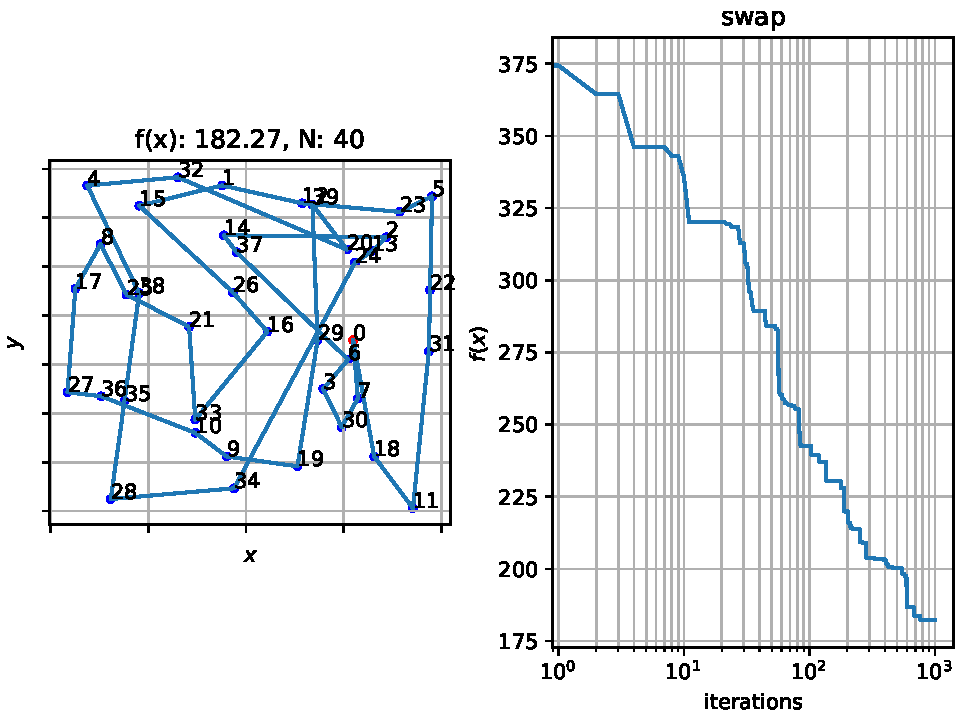
\includegraphics[width=0.49\textwidth]{rand-swap}} \,
\subfloat[\emph{\texttt{reverse} method on random layout}]%
	{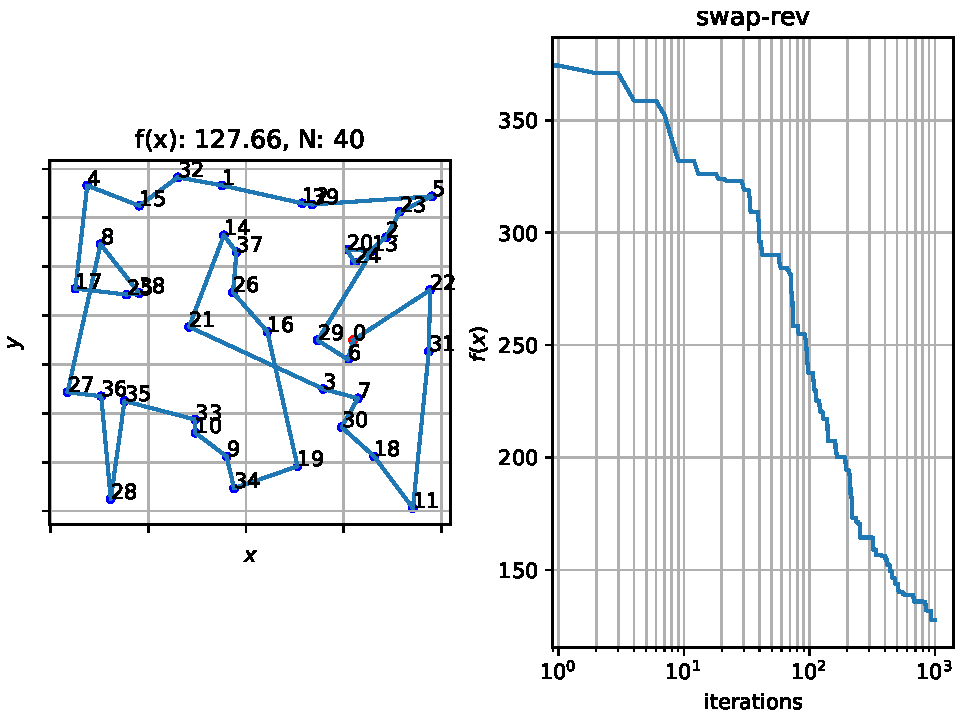
\includegraphics[width=0.49\textwidth]{rand-swaprev}}
\caption{Local search algorithms performance on an instance of the problem}
\label{fig:res-local-search}
\end{figure}

\begin{figure}
\centering
\subfloat[\emph{Circular layout}]%
	{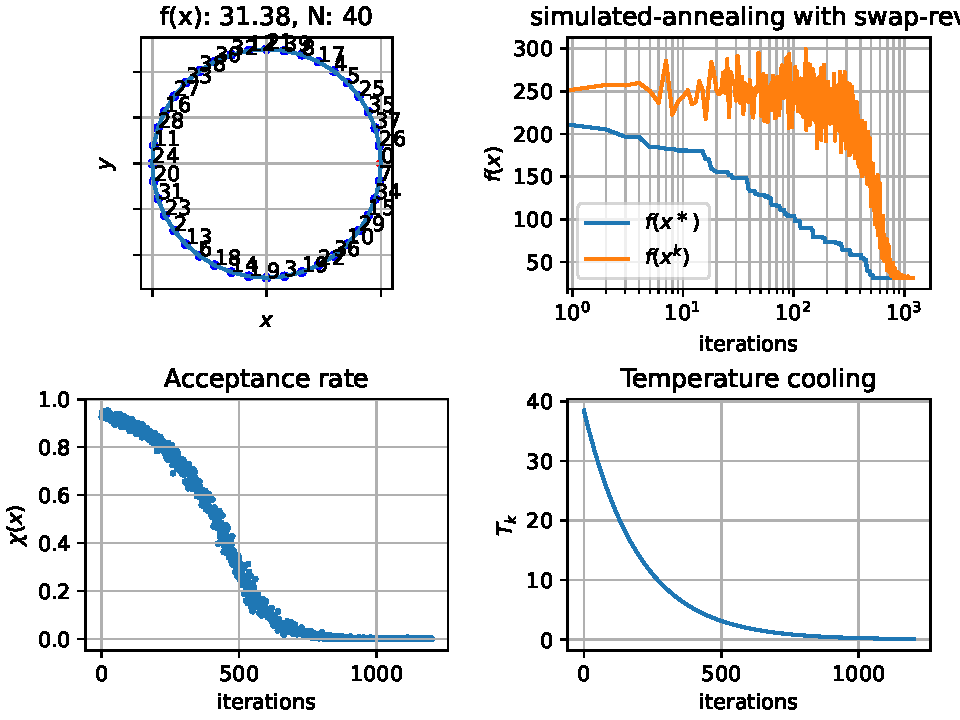
\includegraphics[width=0.49\textwidth]{circle-annealing-quad}} \,
\subfloat[\emph{Random layout}]%
	{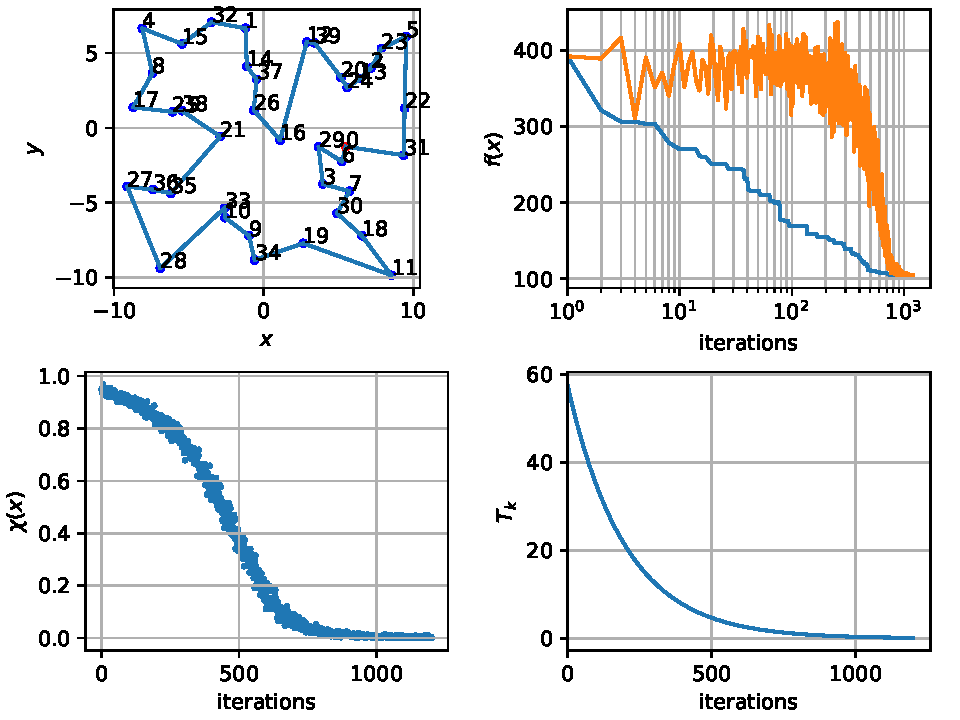
\includegraphics[width=0.49\textwidth]{rand-annealing-quad}}
\caption{Simulated annealing performance on a instance of the problem}
\label{fig:res-sim-annealing}
\end{figure}
